\section{触摸延时开关电路图}
上一节,我们了解了绘制电子电器元件的方法及电子元器件图块的制作方法。这一节中,我们将应用我们所做的电子元器件图块和CAD绘图技巧完成本章开始所展示的触摸延时开关电路图。
\subsection{绘制参考线}
为使绘制的电路图整齐美观,我们要先建立一个参考线图层,并用Xline绘制参考线,以便于电子元件定位。建立图层的方法请参看\ref{sec:falan}图层管理的相关内容,此处不再重复。

\begin{lstlisting}
%命令: xline%
%指定点或 [水平(H)/垂直(V)/角度(A)/二等分(B)/偏移(O)]: 0,0%
%指定通过点:$ @1<0$%
%指定通过点: $@1<90$%
%指定通过点:%
\end{lstlisting}
然后以30mm为间距对参考线进行偏移,形成参考线网格,具体过程在此不再重复,如图\ref{fig:cankaoxian}所示。

\noindent
\begin{figure}[htbp]
\centering
\begin{floatrow}
\ffigbox{\caption{参考线}\label{fig:cankaoxian}}{
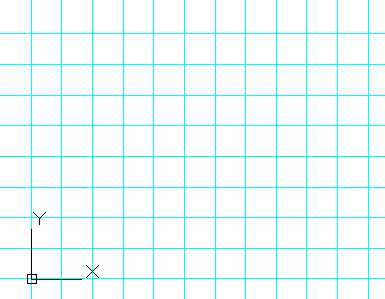
\includegraphics[scale=0.4]{cankaoxian.png}
}
\ffigbox{\caption{块插入}\label{fig:kuaicaru}}{
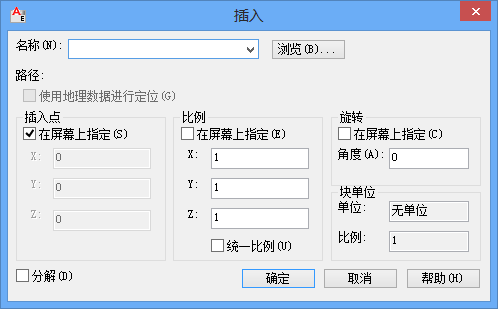
\includegraphics[scale=0.45]{kuaicaru.png}
}
\end{floatrow}
\end{figure}
\subsection{绘制电器元件}
参考线绘制完成后,我们就开始绘制电子元器件,其绘制方法主要是进行块插入操作,即加载相应的电子元器件图块,并将其放到相应的参考线上。

块的插入操作比较简单,当输入insert后好即出现图\ref{fig:kuaicaru}所示对话框,点击【浏览】按钮,找到相应的电子元器件文件并确定,实现元件块调入,接下来填写相应的参数,最后点击确定。

由于块插入操作是一致的,我们在此只以桥式电路元件为例进行演示,其它元件的绘制以此为参照即可,不在鳌述,最络结果如图\ref{fig:onlydianziyujian}所示。
\begin{lstlisting}
%命令:INSERT%
%指定插入点或 [基点(B)/比例(S)/X/Y/Z/旋转(R)]:%
%命令: insert%
%指定插入点或 [基点(B)/比例(S)/X/Y/Z/旋转(R)]: r%
%指定旋转角度 $<0>$: 180%
%指定插入点或 [基点(B)/比例(S)/X/Y/Z/旋转(R)]:%
%命令: insert%
%指定插入点或 [基点(B)/比例(S)/X/Y/Z/旋转(R)]:%
%命令: INSERT%
%指定插入点或 [基点(B)/比例(S)/X/Y/Z/旋转(R)]: r%
%指定旋转角度 $<0>$: 180%
%指定插入点或 [基点(B)/比例(S)/X/Y/Z/旋转(R)]:%
%命令: insert%
%指定插入点或 [基点(B)/比例(S)/X/Y/Z/旋转(R)]:%
\end{lstlisting}
\noindent
\begin{figure}
\centering
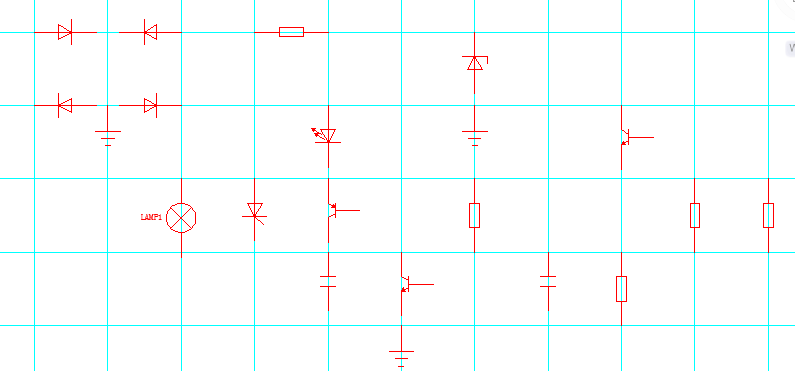
\includegraphics[scale=0.5]{onlydianjiyuanjian.png}
\caption{电路元件图}\label{fig:onlydianziyujian}
\end{figure}
\subsection{绘制线路}
最后,我们根据电路的特点,新建图层并绘水平或垂直连接线即可完成电路图,其过程与图形的绘相同因此就不在一一叙述了。最终结果如图\ref{fig:zhumodianlu}所示。

\zhishi{insert命令解析}
insert命令用于将块或图形插入当前图形中。 其主要选项的含义如下:
\begin{itemize}
\item 基点(B):将块临时放置到当前所在的图形中,并允许在将块参考拖动到位时为其指定新基点。这不会影响为块参照定义的实际基点。 
\item 比例(s):为 X、Y 和 Z 轴设定比例因子。Z 轴比例是指定比例因子绝对值。
\item X:设定 X 比例因子。
\item Y:设定 Y 比例因子。
\item Z:设定 Z 比例因子。
\item 旋转(R):设定块插入的旋转角度。
\end{itemize}

\endinput